% Gemini theme
% https://github.com/anishathalye/gemini

\documentclass[final, 20pt]{beamer}

% ====================
% Packages
% ====================
%\usepackage[x11names]{xcolor} % use color for the horizontal line
\usepackage[T1]{fontenc}
\usepackage{lmodern}
\usepackage[size=custom,width=84.1,height=118.9,scale=1.0]{beamerposter}
\usetheme{gemini}
\usecolortheme{gemini}
\usepackage{graphicx}
\usepackage{booktabs}
\usepackage{tikz}
\usepackage{pgfplots}
\usepackage[square,sort,comma,numbers]{natbib} % for simplify the format of the references
\usepackage{tikz} % for adding the logo


% ====================
% Lengths
% ====================

% If you have N columns, choose \sepwidth and \colwidth such that
% (N+1)*\sepwidth + N*\colwidth = \paperwidth
\newlength{\sepwidth}
\newlength{\colwidth}
\setlength{\sepwidth}{0.025\paperwidth}
\setlength{\colwidth}{0.45\paperwidth}

\newcommand{\separatorcolumn}{\begin{column}{\sepwidth}\end{column}}

% ====================
% Title
% ====================

\title{The day-time patterns of carbohydrate intake \\ in the UK - results from the NDNS RP (2008-16)}

\author{Chaochen Wang \inst{1,2} \and Suzana Almoosawi \inst{3} \and Luigi Palla \inst{1}}

\institute[shortinst]{\inst{1} Dept Medical Statistics, LSHTM, London, UK; \samelineand \inst{2} Dept Public Health, Aichi Medical University, Aichi, Japan \samelineand \\ \inst{3} Brain, Performance and Nutrition Research Centre, Northumbria University, Newcastle, UK}

% ====================
% Body
% ====================
\pgfplotsset{compat=1.16}
\begin{document}

% logos are added as follows:

\addtobeamertemplate{headline}{} 
{
	\begin{tikzpicture}[remember picture,overlay] 
%	\node [anchor=north east, inner sep=3cm] at (current page.north east) {\includegraphics[height=5cm]{Fig/LSHTM-logo-trans-white.eps}}; 
    \node [anchor=north east, inner sep=3cm] at ([xshift=1.4cm,yshift=1.3cm]current page.north east)     {\includegraphics[height=6.5cm]{Fig/LSHTM-logo-trans-white.eps}}; 
	\end{tikzpicture} 
}

\addtobeamertemplate{headline}{} 
{
	\begin{tikzpicture}[remember picture,overlay] 
	%	\node [anchor=north east, inner sep=3cm] at (current page.north east) {\includegraphics[height=5cm]{Fig/LSHTM-logo-trans-white.eps}}; 
	\node [anchor=north west, inner sep=3cm] at ([xshift=-1.5cm,yshift=1.5cm]current page.north west) {\includegraphics[height=7cm]{Fig/amu-logo-trans-white.eps}}; %{\includegraphics[height=6.6cm]{Fig/amu-logo-trans-green.eps}};  
	\end{tikzpicture} 
}

\addtobeamertemplate{headline}{} 
{
	\begin{tikzpicture}[remember picture,overlay] 
	%	\node [anchor=north east, inner sep=3cm] at (current page.north east) {\includegraphics[height=5cm]{Fig/LSHTM-logo-trans-white.eps}}; 
	\node [anchor=north west, inner sep=3cm] at ([xshift=7cm,yshift=1.5cm]current page.north west) {
\includegraphics[height=7cm]{Fig/suzana-logo-trans-white.eps}}; \end{tikzpicture} 
}



\begin{frame}[t]
\begin{columns}[t]
\separatorcolumn

\begin{column}{\colwidth}

  \begin{block}{Introduction}

%The importance of the circadian rhythms has been recognized for long, while its impact on nutrition is still largely unknown. Meal timing has been found to be associated with a wide variety of physiological processes as well as health outcomes: 
The importance of circadian rhythms has long been recognised. However, it remains uncertain whether current dietary guidelines should provide specific recommendations for timing of energy or macro-nutrient intake. Meal timing has been found to be associated with a wide variety of physiological processes as well as health outcomes:
% However, it remains uncertain whether timing of energy or macro-nutrient intake has an impact on health or disease.
    \vskip-1.45ex
    \begin{itemize}
	\item Skipping breakfast is associated with a higher risk of developing type 2 diabetes (T2D) \cite{uemura2015breakfast};
	\item Replacing fat at breakfast with carbohydrate is associated with lower risk of T2D incidence \cite{almoosawi2013diurnal};
	\item Evening intake of energy is positively associated with incidence of hypertension, and overweight/obesity \cite{Almoosawi2013,almoosawi2016chrono}.
%	\item Shift workers have a higher risk of developing T2D \cite{pan2011rotating}. 
    \end{itemize}
    \vskip-1.45ex

Recent evidence suggested that there are three types of eaters \textbf{(grazers, early eaters, and late eaters)} according to the timing of energy consumption \cite{leech2017temporal,mansukhani2018investigating}. However, the temporal eating patterns were based on averaging the total energy intake  measured in the questionnaires and therefore \textbf{could not capture the day-to-day variation in eating patterns}. Furthermore, most previous studies have focused on describing temporal patterns of energy intake, \textbf{without considering the timing of macro-nutrient intake}.

%    \vskip-1.45ex
%%\begin{itemize}
%	\item 
%	\item 
%	
%%	Besides they were focussed on total energy \textbf{so would not provide any clue of the temporal eating patterns specifically for nutrient intake}.
%	%	\item Shift workers have a higher risk of developing T2D \cite{pan2011rotating}. 
%%\end{itemize}
%\vskip-1.45ex

%%
%However, the temporal eating patterns were based only on averaging the total energy intake measured by 1 or 2 24-hour dietary recalls \cite{leech2017temporal} or 3 to 4 days' diet diary \cite{mansukhani2018investigating} and therefore \textbf{could not capture the day-to-day variation in eating patterns}, and \textbf{neither could it provide any clue of the temporal patterns specifically for nutrient intake}. 

%This is mainly due to limitations in the FFQ often used in observational studies and the lack of understanding of statistical techniques that can capture the complexity of eating patterns across the day. 

This study aims at finding both time and quantity eating patterns specifically for carbohydrate (CH) intake in UK adults.


  \end{block}


   \vskip-1.85ex
  \begin{block}{Data and Methodology}
    \vskip-1.85ex
\begin{itemize}
	\item Data from the National Diet and Nutrition Survey (NDNS) Rolling Programme (2008/09-15/16) included 6155 adults (2537 men and 3618 women) aged 19 or older in the UK. 
	\item Time of the day was categorised into 7 slots: 6-9 am, 9-12 noon, 12-2 pm, 2-5 pm, 5-8 pm, 8-10 pm and 10 pm-6 am. 
	\item Responses for CH intake within each time slot were categorised into: 1) no energy intake, 2) CH contributed  $<$ 50\%, or 3) CH contributed $\geqslant$ 50\% of total energy. 
	\item Multilevel latent class analysis (MLCA) models \cite{finch2017multilevel} were applied to explore latent classes of CH consumption, accounting for the repeated measurement of intake over 3-4 days nested within individuals. 
%	\item Survey-designed multivariable regression models were used to assess the associations of CH eating patterns with hypertension and obesity.
\end{itemize}
    \vskip-1.45ex
  \end{block}
\end{column}

\separatorcolumn

\begin{column}{\colwidth}

%   \vskip-0.85ex
  \begin{block}{Results}
%\heading{Day Level Carbohydrate Eating Patterns}
\heading{Day Level Carbohydrate Eating Patterns}
	Three CH eating day patterns emerged from 24483 observation days \textbf{(Fig. \ref{fig:daylevel})}.  
      \vskip-1.9ex
    \begin{figure}
      \centering
      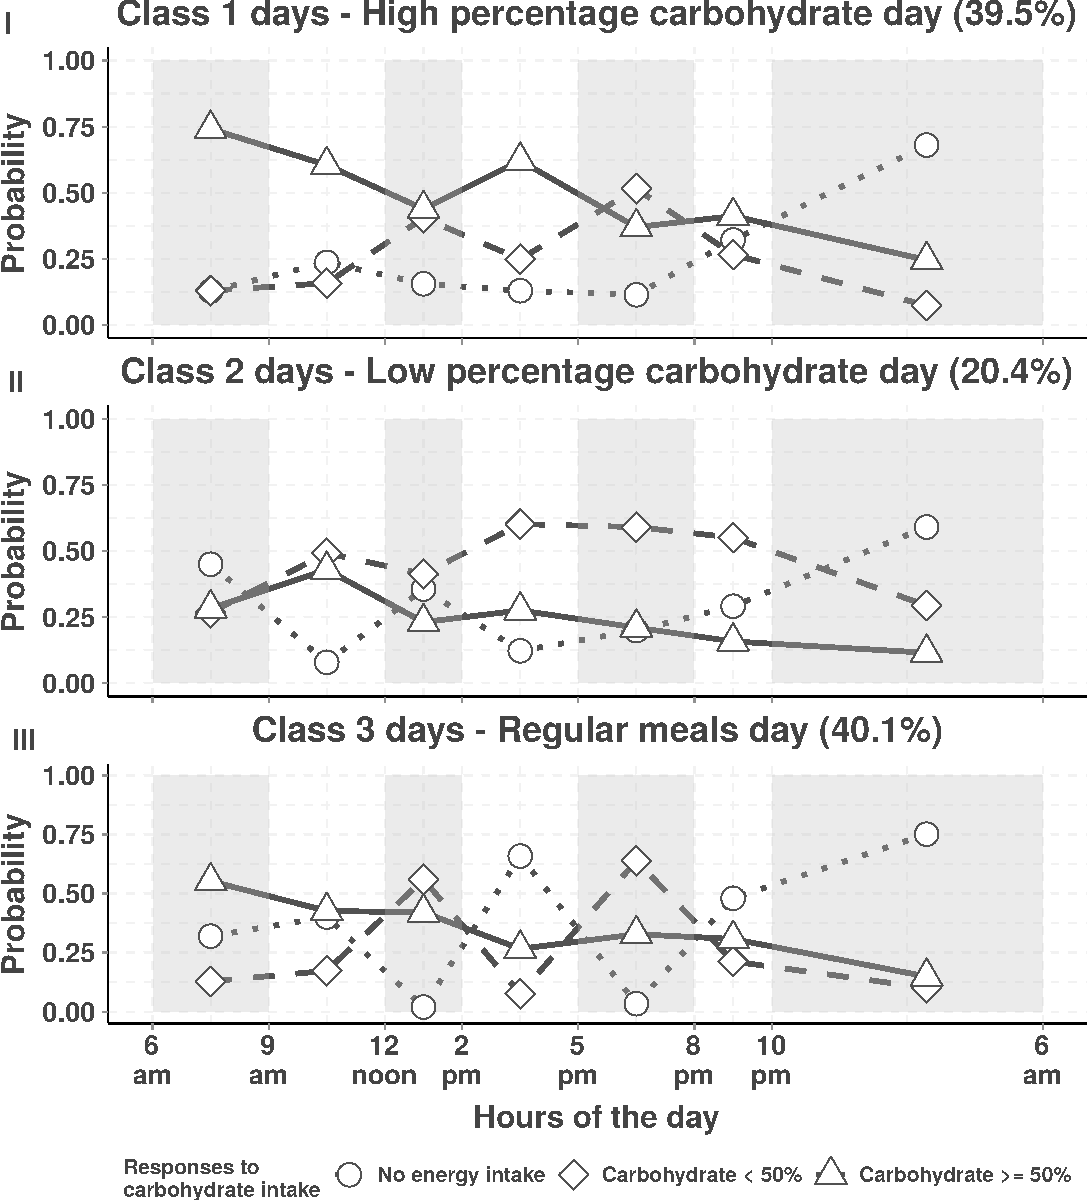
\includegraphics[width=0.65\textwidth]{Fig/Fig01.eps}	\vskip-2.45ex
      \caption{Day level latent class solutions (Class 1-3 days).}
      \label{fig:daylevel}
    \end{figure}
\vskip-1.9ex
%  \end{block}


\heading{Individual Level Latent Class Solution}
%  \begin{block}{Individual Level Latent Class Solution}
%	\vskip-2.45ex
Based on the distribution of CH day patterns among the individuals, three types of CH eaters were defined which could be broadly labelled as low (28.1\%), moderate (28.8\%), and high (43.1\%) CH eaters \textbf{(Fig. \ref{fig:indilevel})}.
      \vskip-2.45ex
	\begin{figure}
	\centering
	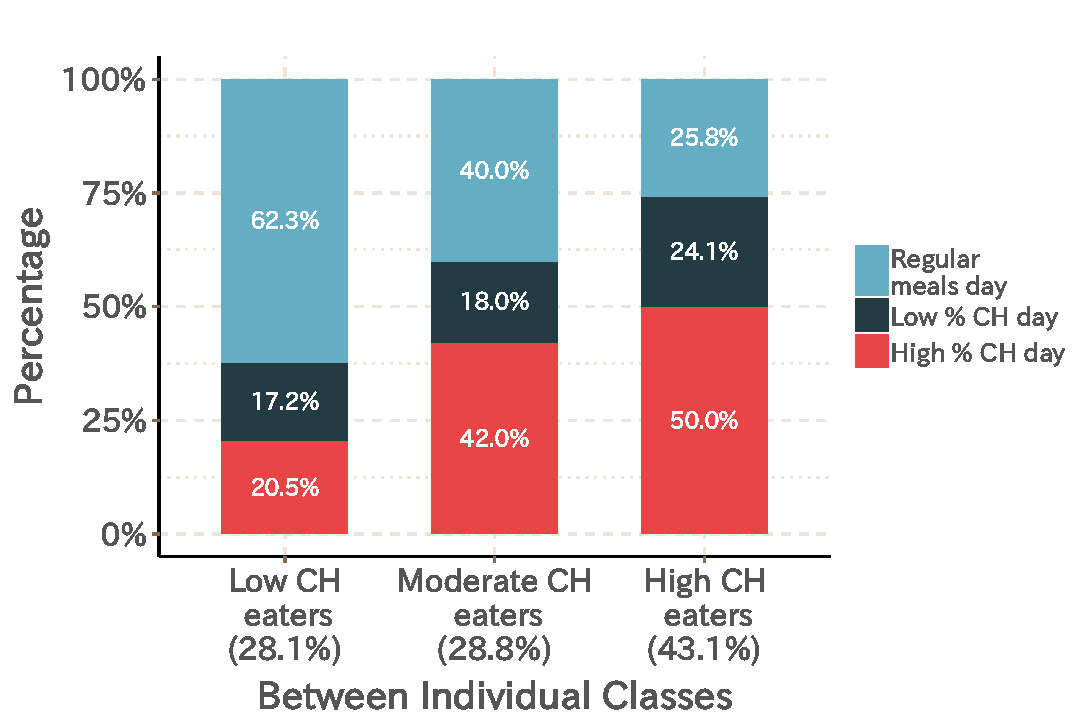
\includegraphics[width=0.6\textwidth]{Fig/level2.eps}	\vskip-2.45ex
	\caption{Multilevel Latent Class Solution, 3 classes in day level, 3 classes in individual level.}
	\label{fig:indilevel}
	\vskip-2.45ex
\end{figure}
%\vskip-1.9ex

  \end{block}


%\begin{block}{Discussion}
%
%\end{block}


\end{column}

\separatorcolumn
\end{columns}


%\heading{Nutrient Contributions to Energy within Time Slots}
%  \begin{block}{}
	%\heading{Day Level Carbohydrate Eating Patterns}
	\vskip-1.8ex
	\begin{figure}
		\centering
%		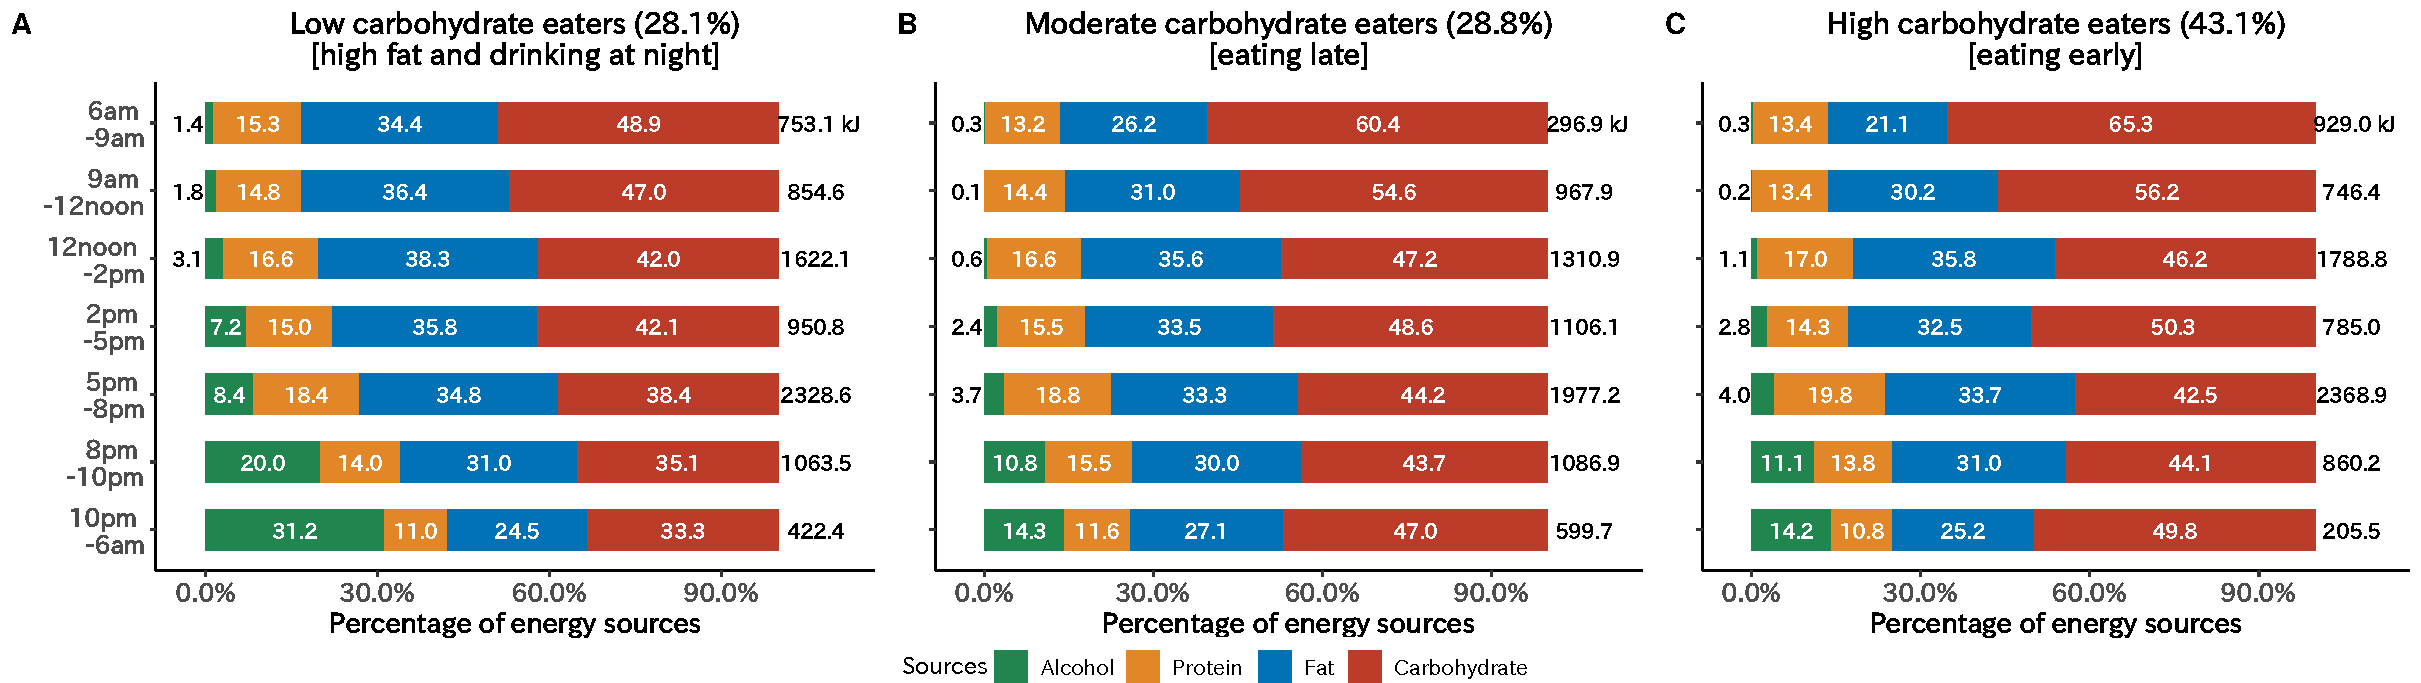
\includegraphics[width=40cm]{Fig/compo.eps}
		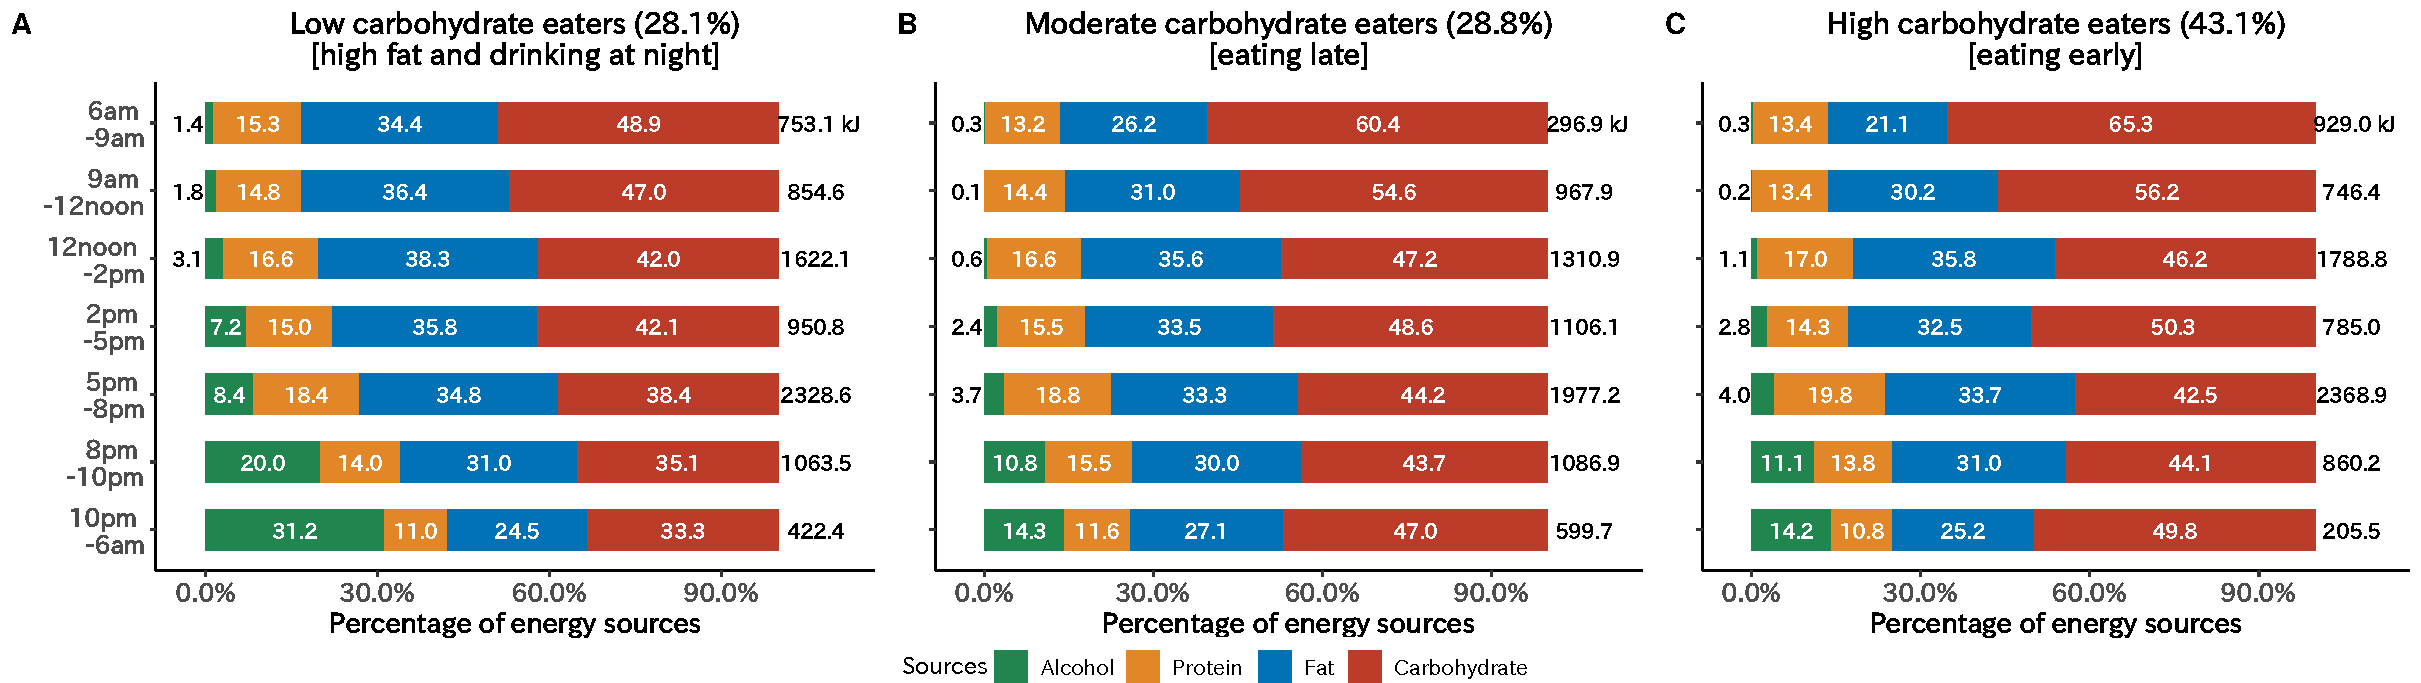
\includegraphics[width=0.8\textwidth]{Fig/compo.eps}\vskip-1.45ex
		      \caption{\textbf{The compositions of energy consumption within each time slot by CH eaters.}}
		      \label{fig:compo}
	\end{figure}\vskip-1.45ex
%\end{block}

%\parbox{0.95\textwidth}{\somebody{On average, low-CH eaters (Fig. \ref{fig:compo}-A) consumed the highest amount of total energy intake (7985.8 kJm \textit{p} < 0.001), and they had higher percentages of energy contributed by fat and alcohol, especially after 8 pm. }}
\par
\begingroup
\leftskip2em
\rightskip\leftskip
\somebody{On average, low-CH eaters \textbf{(Fig. \ref{fig:compo}-A)} consumed the highest amount of total energy intake (7985.8 kJ, \textit{p} < 0.001), and they had higher percentages of energy contributed by fat and alcohol, especially after 8 pm. Moderate-CH eaters \textbf{(Fig. \ref{fig:compo}-B)} consumed the lowest amount of total energy (7341.8 kJ) while they had the tendency of eating later in the day. High-CH eaters \textbf{(Fig. \ref{fig:compo}-C)} consumed most of their CH and energy within time slots of 6-9 am, 12-2 pm, and 5-8 pm.}
\par
\endgroup

\someheading{Discussion}
\par
\begingroup
\leftskip2em
\rightskip\leftskip
\somebody{The high-CH eaters profile seemed to be the healthiest. Low-CH eating which was crudely associated with higher prevalence of hypertension and obesity may have resulted from health/weight concerns, leading to fat or alcohol as replacements for CH. To ascertain the direction of causality in the association of CH patterns with blood pressure and obesity, prospective longitudinal studies are warranted. }
\par
\endgroup

\noindent\textcolor{steelblue}{\rule{\textwidth}{0.4pt}}
%  \begin{block}{References}
    \vskip-1.25ex
%    \nocite{*}
    \footnotesize{\bibliographystyle{elsarticle-num}\bibliography{poster.bib}}

%  \end{block}

%\end{column}
%
%\separatorcolumn
%\end{columns}
%\end{frame}
\end{frame}
\end{document}
